%CS-113 S18 HW-2
%Released: 2-Feb-2018
%Deadline: 16-Feb-2018 7.00 pm
%Authors: Abdullah Zafar, Emad bin Abid, Moonis Rashid, Abdul Rafay Mehboob, Waqar Saleem.


\documentclass[addpoints]{exam}

% Header and footer.
\pagestyle{headandfoot}
\runningheadrule
\runningfootrule
\runningheader{CS 113 Discrete Mathematics}{Homework II}{Spring 2018}
\runningfooter{}{Page \thepage\ of \numpages}{}
\firstpageheader{}{}{}

\boxedpoints
\printanswers
\usepackage[table]{xcolor}
\usepackage{amsfonts,graphicx,amsmath,hyperref}
\title{Habib University\\CS-113 Discrete Mathematics\\Spring 2018\\HW 2}
\author{$<your ID>$}  % replace with your ID, e.g. oy02945
\date{Due: 19h, 16th February, 2018}


\begin{document}
\maketitle

\begin{questions}



\question

%Short Questions (25)

\begin{parts}

  
  \part[5] Determine the domain, codomain and set of values for the following function to be 
  \begin{subparts}
  \subpart Partial
  \subpart Total
  \end{subparts}
  \begin{center}
    $y=\sqrt{x}$
  \end{center}

  \begin{solution}
    % Write your solution here
  \end{solution}
  
  \part[5] Explain whether $f$ is a function from the set of all bit strings to the set of integers if $f(S)$ is the smallest $i \in \mathbb{Z}$� such that the $i$th bit of S is 1 and $f(S) = 0$ when S is the empty string. 
  
  \begin{solution}
    % Write your solution here
  \end{solution}

  \part[15] For $X,Y \in S$, explain why (or why not) the following define an equivalence relation on $S$:
  \begin{subparts}
    \subpart ``$X$ and $Y$ have been in class together"
    \subpart ``$X$ and $Y$ rhyme"
    \subpart ``$X$ is a subset of $Y$"
  \end{subparts}

  \begin{solution}
    % Write your solution here
  \end{solution}

\end{parts}

%Long questions (75)
\question[15] Let $A = f^{-1}(B)$. Prove that $f(A) \subseteq B$.
  \begin{solution}
    % Write your solution here
  \end{solution}

\question[15] Consider $[n] = \{1,2,3,...,n\}$ where $n \in \mathbb{N}$. Let $A$ be the set of subsets of $[n]$ that have even size, and let $B$ be the set of subsets of $[n]$ that have odd size. Establish a bijection from $A$ to $B$, thereby proving $|A| = |B|$. (Such a bijection is suggested below for $n = 3$) 

\begin{center}

  \begin{tabular}{ |c || c | c | c |c |}
    \hline
 A & $\emptyset$ & $\{2,3\}$ & $\{1,3\}$ & $\{1,2\}$ \\ \hline
 B & $\{3\}$ & $\{2\}$ & $\{1\}$ & $\{1,2,3\}$\\\hline
\end{tabular}
\end{center}

  \begin{solution}
    % Write your solution here
  \end{solution}
  
\question Mushrooms play a vital role in the biosphere of our planet. They also have recreational uses, such as in understanding the mathematical series below. A mushroom number, $M_n$, is a figurate number that can be represented in the form of a mushroom shaped grid of points, such that the number of points is the mushroom number. A mushroom consists of a stem and cap, while its height is the combined height of the two parts. Here is $M_5=23$:

\begin{figure}[h]
  \centering
  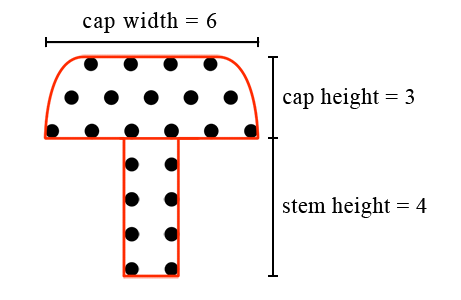
\includegraphics[scale=1.0]{m5_figurate.png}
  \caption{Representation of $M_5$ mushroom}
  \label{fig:mushroom_anatomy}
\end{figure}

We can draw the mushroom that represents $M_{n+1}$ recursively, for $n \geq 1$:
\[ 
    M_{n+1}=
    \begin{cases} 
      f(\textrm{Cap\_width}(M_n) + 1, \textrm{Stem\_height}(M_n) + 1, \textrm{Cap\_height}(M_n))  & n \textrm{ is even} \\
      f(\textrm{Cap\_width}(M_n) + 1, \textrm{Stem\_height}(M_n) + 1, \textrm{Cap\_height}(M_n)+1) & n \textrm{ is odd}  \\      
   \end{cases}
\]

Study the first five mushrooms carefully and make sure you can draw subsequent ones using the recurrence above.

\begin{figure}[h]
  \centering
  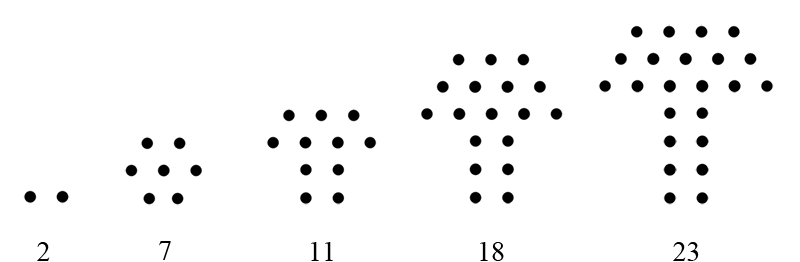
\includegraphics{mushroom_series.png}
  \caption{Representation of $M_1,M_2,M_3,M_4,M_5$ mushrooms}
  \label{fig:mushroom_anatomy}
\end{figure}

  \begin{parts}
    \part[15] Derive a closed-form for $M_n$ in terms of $n$.
  \begin{solution}
    % Write your solution here
  \end{solution}
    \part[5] What is the total height of the $20$th mushroom in the series? 
  \begin{solution}
    % Write your solution here
  \end{solution}
\end{parts}

\question
    The \href{https://en.wikipedia.org/wiki/Fibonacci_number}{Fibonacci series} is an infinite sequence of integers, starting with $1$ and $2$ and defined recursively after that, for the $n$th term in the array, as $F_n = F_{n-1} + F_{n-2}$. In this problem, we will count an interesting set derived from the Fibonacci recurrence.
    
The \href{http://www.maths.surrey.ac.uk/hosted-sites/R.Knott/Fibonacci/fibGen.html#section6.2}{Wythoff array} is an infinite 2D-array of integers where the $n$th row is formed from the Fibonnaci recurrence using starting numbers $n$ and $\left \lfloor{\phi\cdot (n+1)}\right \rfloor$ where $n \in \mathbb{N}$ and $\phi$ is the \href{https://en.wikipedia.org/wiki/Golden_ratio}{golden ratio} $1.618$ (3 sf).

\begin{center}
\begin{tabular}{c c c c c c c c}
 \cellcolor{blue!25}1 & 2 & 3 & 5 & 8 & 13 & 21 & $\cdots$\\
 4 & \cellcolor{blue!25}7 & 11 & 18 & 29 & 47 & 76 & $\cdots$\\
 6 & 10 & \cellcolor{blue!25}16 & 26 & 42 & 68 & 110 & $\cdots$\\
 9 & 15 & 24 & \cellcolor{blue!25}39 & 63 & 102 & 165 & $\cdots$ \\
 12 & 20 & 32 & 52 & \cellcolor{blue!25}84 & 136 & 220 & $\cdots$ \\
 14 & 23 & 37 & 60 & 97 & \cellcolor{blue!25}157 & 254 & $\cdots$\\
 17 & 28 & 45 & 73 & 118 & 191 & \cellcolor{blue!25}309 & $\cdots$\\
 $\vdots$ & $\vdots$ & $\vdots$ & $\vdots$ & $\vdots$ & $\vdots$ & $\vdots$ & \color{blue}$\ddots$\\
 

\end{tabular}
\end{center}

\begin{parts}
  \part[10] To begin, prove that the Fibonacci series is countable.
 
    \begin{solution}
    % Write your solution here
  \end{solution}
  \part[15] Consider the Modified Wythoff as any array derived from the original, where each entry of the leading diagonal (marked in blue) of the original 2D-Array is replaced with an integer that does not occur in that row. Prove that the Modified Wythoff Array is countable. 

  \begin{solution}
    % Write your solution here
  \end{solution}
\end{parts}

\end{questions}

\end{document}